\documentclass[12pt,a4paper]{article}

% ================================================================
% ARTIGO -- ANÁLISE DE DESEMPENHO DE UMA FILA M/M/1
% Estrutura baseada na ABNT NBR 6022 e nas orientações da UNIFAL-MG.
% Para usar no Overleaf, mantenha este arquivo na raiz do projeto e
% os arquivos gráficos dentro da pasta "imagens".
% ================================================================

% ---------- Idioma e fonte ----------
\usepackage[T1]{fontenc}
\usepackage[utf8]{inputenc}
\usepackage[brazilian]{babel}
\usepackage{lmodern}
\usepackage{microtype}

% ---------- Página e parágrafos ----------
\usepackage{geometry}
\geometry{
  top=3cm,
  bottom=2cm,
  left=3cm,
  right=2cm
}
\usepackage{setspace}
\onehalfspacing
\usepackage{indentfirst}
\setlength{\parindent}{1.25cm}
\setlength{\parskip}{0pt}

% ---------- Matemática, figuras e tabelas ----------
\usepackage{amsmath,amssymb}
\usepackage{graphicx}
\graphicspath{{imagem/}}
\usepackage{booktabs}
\usepackage{tabularx}
\usepackage{float}
\usepackage{caption}
\captionsetup{
  font=small,
  labelfont=bf,
  justification=centering
}

% ---------- Links ----------
\usepackage[hidelinks]{hyperref}
\usepackage{url}

% ---------- Numeração de páginas ----------
\usepackage{fancyhdr}
\pagestyle{fancy}
\fancyhf{}
\fancyhead[R]{\thepage}
\renewcommand{\headrulewidth}{0pt}
\setlength{\headheight}{14.5pt}

% ---------- Comandos usados no texto ----------
\newcommand{\EN}{\mathrm{E}[N]}
\newcommand{\EW}{\mathrm{E}[W]}
\newcommand{\ENq}{\mathrm{E}[N_q]}
\newcommand{\EWq}{\mathrm{E}[W_q]}

\begin{document}

% ================================================================
% ELEMENTOS PRÉ-TEXTUAIS
% ================================================================

\begin{center}
  {\large\bfseries
  MODELAGEM E SIMULAÇÃO DE UMA FILA M/M/1: ANÁLISE DE DESEMPENHO EM DIFERENTES CENÁRIOS
  \par}

  \vspace{0.7cm}

  {\normalsize Jeann Victor Batista\par}
  \vspace{0.2cm}
  {\small Universidade Federal de Alfenas -- UNIFAL-MG\par}
  {\small Bacharelado em Ciência da Computação\par}
  {\small Disciplina: Análise de Desempenho\par}
  {\small Professor: Flávio Barbieri Gonzaga\par}
\end{center}

\vspace{0.7cm}

\begin{spacing}{1.0}
\noindent\textbf{Resumo:}
Este trabalho analisa um simulador a eventos discretos de uma fila M/M/1 implementado em linguagem C, relacionando seu funcionamento à notação de Kendall, à estabilidade e à Lei de Little. Foram avaliados sete cenários, com intensidades de tráfego entre 0,25 e 1,10, quatro horizontes e 30 repetições por configuração, totalizando 840 execuções da versão original adaptada para testes em lote e 840 de uma versão com correções básicas. Como contribuição metodológica, o estudo combina comparação teórica, intervalos de confiança, conservação de fluxo e análise pareada para distinguir variabilidade amostral de efeitos da implementação. Nos cenários estáveis, as médias aproximaram-se dos valores teóricos com o aumento do horizonte. Para $T=10^5$, os erros relativos ficaram abaixo de 0,4\% nos três primeiros cenários e chegaram a aproximadamente 2,35\% nas cargas próximas da saturação. Nos cenários crítico e sobrecarregado, observaram-se crescimento da população final e vazão próxima da capacidade do servidor. A versão original ultrapassou o horizonte solicitado, mas o efeito relativo desse problema diminuiu nas execuções longas. O resíduo de Little foi próximo de zero por construção algébrica, o que limita seu uso como validação independente. Os resultados sustentam a coerência do simulador nas condições avaliadas e mostram que a proximidade da saturação exige maior duração e cuidado na interpretação.

\vspace{0.3cm}
\noindent\textbf{Palavras-chave:}
teoria de filas; simulação a eventos discretos; M/M/1; Lei de Little; análise de desempenho.
\end{spacing}

% ================================================================
% 1 INTRODUÇÃO
% ================================================================

\section{Introdução}

Em sistemas computacionais, diferentes recursos podem receber solicitações em uma velocidade superior àquela com que conseguem processá-las. Quando o atendimento não ocorre imediatamente, as solicitações permanecem no sistema e formam filas. Esse comportamento está presente, por exemplo, em servidores, roteadores, processadores e sistemas de armazenamento. A análise dessas filas permite compreender como a carga de trabalho influencia a utilização dos recursos, a quantidade de solicitações presentes e o tempo necessário para concluir cada atendimento.

A teoria de filas e a simulação a eventos discretos constituem formas complementares de estudar esses sistemas. A teoria fornece expressões matemáticas para medidas de desempenho sob determinadas hipóteses, enquanto a simulação reproduz computacionalmente a evolução do sistema e permite observar seu comportamento em condições variadas. Entre os modelos clássicos está a fila M/M/1, caracterizada por intervalos entre chegadas exponenciais, tempos de atendimento exponenciais e um único servidor (TRIVEDI, 2001). A comparação entre teoria e simulação também auxilia na identificação de limitações ou erros de implementação (ROSS, 2006).

Este trabalho parte do arquivo \texttt{simulacao\_v3.c}, fornecido na disciplina de Análise de Desempenho. O programa gera eventos de chegada e saída, controla a quantidade de solicitações no sistema e calcula ocupação, número médio de solicitações e tempo médio de permanência. A análise examina a influência da carga e da duração das execuções, a variabilidade entre repetições, a conservação do fluxo e o comportamento dos regimes crítico e sobrecarregado. Também investiga o efeito de correções básicas no encerramento da simulação.

O objetivo é analisar o desempenho da fila em diferentes cenários e verificar em que condições os resultados experimentais se aproximam das previsões do modelo M/M/1. Para isso, são empregados a notação de Kendall, a condição de estabilidade, as fórmulas de regime estacionário e a Lei de Little. O estudo compara a versão V3, mantida com sua lógica original, e a versão V4, que corrige problemas de entrada e de encerramento sem introduzir novas medidas de desempenho. Tabelas, intervalos de confiança e gráficos são utilizados para organizar e discutir os resultados.

O artigo está organizado da seguinte forma: a seção 2 apresenta a fundamentação teórica; a seção 3 descreve o código e suas limitações; a seção 4 detalha o experimento e o tratamento estatístico; a seção 5 discute os resultados; e a seção 6 apresenta as considerações finais.

% ================================================================
% 2 FUNDAMENTAÇÃO TEÓRICA
% ================================================================

\section{Fundamentação teórica}

\subsection{Processos de chegada e distribuição exponencial}

No modelo M/M/1, considera-se que as chegadas formam um processo de Poisson de taxa $\lambda>0$. Assim, a quantidade $C(t)$ de chegadas observadas em um intervalo de duração $t$ possui distribuição de Poisson:
\begin{equation}
  P\{C(t)=k\}=e^{-\lambda t}\frac{(\lambda t)^k}{k!},
  \qquad k=0,1,2,\ldots
  \label{eq:poisson}
\end{equation}
O parâmetro $\lambda$ representa a quantidade média de chegadas por unidade de tempo. Por exemplo, $\lambda=0{,}5$ solicitação por segundo corresponde, no longo prazo, a uma chegada a cada dois segundos.

Os intervalos $X$ entre chegadas consecutivas são independentes e seguem uma distribuição exponencial de taxa $\lambda$, cuja função de distribuição acumulada é
\begin{equation}
  F_X(x)=P\{X\leq x\}=1-e^{-\lambda x},
  \qquad x\geq 0.
  \label{eq:exponencial-chegada}
\end{equation}
O intervalo médio entre chegadas é $\mathrm{E}[X]=1/\lambda$. De maneira semelhante, o tempo de atendimento $S$ é exponencial de taxa $\mu$ e possui média $\mathrm{E}[S]=1/\mu$. A distribuição exponencial apresenta ausência de memória, propriedade que permite representar o sistema como um processo markoviano (TRIVEDI, 2001; GONZAGA, 2026).

\subsection{Geração de variáveis pela transformada inversa}

O simulador gera intervalos exponenciais pelo método da transformada inversa. A partir de uma variável pseudoaleatória uniforme $U$ no intervalo $(0,1]$, uma amostra exponencial de taxa $r$ é obtida por
\begin{equation}
  X=-\frac{\ln(U)}{r}.
  \label{eq:transformada-inversa}
\end{equation}
No código, usa-se $r=\lambda$ para o tempo até a próxima chegada e $r=\mu$ para a duração do atendimento. A função \texttt{aleatorio()} produz $U$, e as expressões que contêm \texttt{log(aleatorio())} implementam a Equação~\ref{eq:transformada-inversa}.

O programa recebe tempos médios, mas os converte internamente em taxas. Se o tempo médio entre chegadas informado for $m_c$, calcula-se $\lambda=1/m_c$; se o tempo médio de atendimento for $m_s$, calcula-se $\mu=1/m_s$. Por isso, apesar dos nomes das variáveis no código, depois da conversão elas passam a armazenar taxas.

\subsection{Notação de Kendall e modelo M/M/1}

A notação de Kendall classifica um sistema de filas pela forma $A/S/c$, em que $A$ representa a distribuição dos intervalos entre chegadas, $S$ representa a distribuição dos tempos de serviço e $c$ indica a quantidade de servidores (KENDALL, 1953). 

No modelo M/M/1, o primeiro M indica intervalos entre chegadas exponenciais, o segundo M indica tempos de atendimento exponenciais e o número 1 indica um único servidor. Sob as hipóteses usuais adotadas neste estudo, a descrição completa é M/M/1/$\infty$/$\infty$/FCFS: capacidade ilimitada, população potencialmente infinita e atendimento na ordem de chegada (\textit{first come, first served}). Também se pressupõe independência entre os intervalos de chegada e os tempos de atendimento.

No código estudado, os dois símbolos M correspondem às chamadas da transformação inversa usadas para programar chegadas e saídas. O número 1 é representado pela existência de apenas um instante de saída agendado. Como o programa trabalha com medidas agregadas e processa um atendimento por vez, a ordem FCFS é implícita, embora não sejam mantidos registros individuais das solicitações.

\subsection{Utilização e condição de estabilidade}

A intensidade de tráfego, também chamada de utilização, é definida por
\begin{equation}
  \rho=\frac{\lambda}{\mu}.
  \label{eq:rho}
\end{equation}
Em uma fila M/M/1 estável, $\rho$ corresponde à fração de tempo em que o servidor permanece ocupado. A existência de um regime estacionário com médias finitas exige
\begin{equation}
  \lambda<\mu \quad\Longleftrightarrow\quad \rho<1.
  \label{eq:estabilidade}
\end{equation}
Quando $\rho$ se aproxima de 1, resta pouca capacidade livre e aumentam a população no sistema, o tempo de permanência e a variabilidade. Para $\rho\geq1$, não existe distribuição estacionária de probabilidade. No caso crítico, $\rho=1$, o processo é recorrente nulo: pode retornar ao estado vazio, mas não possui um equilíbrio estacionário normalizável. Quando $\rho>1$, o processo é transiente e a demanda excedente produz crescimento persistente da população. Uma execução limitada ainda fornece valores numéricos, que dependem do horizonte e não devem ser interpretados como médias de equilíbrio (TRIVEDI, 2001).

\subsection{Medidas de desempenho do M/M/1}

Seja $N(t)$ a quantidade de solicitações no sistema no instante $t$, incluindo a que está em atendimento. Sua média estacionária é $L=\mathrm{E}[N]$. A quantidade média apenas na fila é $L_q$. De modo análogo, $W$ representa o tempo médio total no sistema e $W_q$ representa apenas o tempo médio de espera antes do atendimento.

Para uma fila M/M/1 estável, essas medidas são dadas por
\begin{equation}
  L=\frac{\rho}{1-\rho}=\frac{\lambda}{\mu-\lambda},
  \qquad L_q=\frac{\rho^2}{1-\rho}.
  \label{eq:l-lq}
\end{equation}
\begin{equation}
  W=\frac{1}{\mu-\lambda},
  \qquad W_q=\frac{\rho}{\mu-\lambda}.
  \label{eq:w-wq}
\end{equation}
As saídas das versões V3 e V4 são estimativas de ocupação, $L$ e $W$. A estimativa de $L$ é temporal, enquanto a de $W$ é indireta e inclui permanências truncadas, conforme discutido na seção 3.5. As grandezas $L_q$ e $W_q$ completam a caracterização teórica, mas não foram incluídas na comparação experimental. Embora $L_q$ possa ser derivado de $L$ e da ocupação quando ambos são medidos corretamente na mesma janela, a subtração $W-1/\mu$ não resolve as limitações do estimador de permanência em um horizonte finito.

\subsection{Lei de Little}

A Lei de Little relaciona a quantidade média de elementos, a taxa efetiva de fluxo e o tempo médio de permanência em um sistema estável (LITTLE, 1961). Para o sistema completo,
\begin{equation}
  L=\EN=\lambda_{\mathrm{ef}}\EW,
  \label{eq:little-sistema}
\end{equation}
em que $\lambda_{\mathrm{ef}}$ é a taxa efetiva de solicitações que atravessam o sistema. Sem perdas ou bloqueios e em regime estável, essa taxa coincide com a taxa externa de chegada $\lambda$. Para a fila de espera,
\begin{equation}
  L_q=\ENq=\lambda_{\mathrm{ef}}\EWq.
  \label{eq:little-fila}
\end{equation}

Intuitivamente, a quantidade média presente equivale à quantidade que entra por unidade de tempo multiplicada pelo tempo médio de permanência. A lei é mais geral que o modelo M/M/1 e não depende de distribuições exponenciais. Entretanto, no programa original, $\EN$ e $\EW$ são derivados das mesmas áreas acumuladas. Assim, o resíduo de Little quase nulo verifica a consistência algébrica interna, mas não constitui, isoladamente, uma validação independente. Neste trabalho, essa verificação é complementada pela comparação teórica e pela análise da taxa de chegada e da vazão.

% ================================================================
% 3 ANÁLISE DO CÓDIGO-FONTE
% ================================================================

\section{Análise do simulador em linguagem C}

\subsection{Visão geral do simulador}

O arquivo \texttt{simulacao\_v3.c} implementa uma simulação a eventos discretos de uma fila com um servidor. O relógio não avança em passos fixos: ele é deslocado diretamente para a próxima chegada ou saída. Essa estratégia evita processar períodos nos quais o estado não muda e é adequada à representação de filas (ROSS, 2006).

O programa recebe o tempo médio entre chegadas, o tempo médio de atendimento e a duração desejada. Os dois primeiros valores são convertidos em taxas e usados para gerar amostras exponenciais. Durante a execução, são mantidos o relógio, a quantidade de solicitações e os instantes da próxima chegada e da próxima saída. Ao final, o programa apresenta ocupação, $\EN$, $\EW$ e o resíduo da Lei de Little.

As estruturas do tipo \texttt{Info} acumulam áreas no tempo. Uma representa $N(t)$; as outras duas representam os processos acumulados de chegada e de saída. Dessa forma, o programa obtém médias temporais sem registrar o estado em todos os instantes.

\subsection{Estado do sistema e escolha do próximo evento}

O relógio é armazenado em \texttt{tempo\_decorrido}. A próxima chegada é registrada em \texttt{chegada\_cliente}; a próxima saída, em \texttt{saida\_cliente}. A variável \texttt{fila} representa a população total no sistema, e não apenas quem aguarda: zero significa servidor ocioso, um significa uma solicitação em atendimento e valores maiores que um indicam espera.

\begin{table}[H]
  \centering
  \caption{Correspondência entre as grandezas do modelo e as variáveis da V3.}
  \label{tab:mapeamento}
  \begin{tabularx}{\textwidth}{@{}lX@{}}
    \toprule
    Grandeza & Variável ou acumulador \\
    \midrule
    Relógio $t$ & \texttt{tempo\_decorrido} \\
    População $N(t)$ & \texttt{fila} e \texttt{en.numero\_eventos} \\
    Próxima chegada & \texttt{chegada\_cliente} \\
    Próxima saída & \texttt{saida\_cliente}, consultada quando há atendimento \\
    Taxa $\lambda$ & \texttt{intervalo\_chegadas}, após a conversão da entrada \\
    Taxa $\mu$ & \texttt{media\_atendimento}, após a conversão da entrada \\
    Chegadas $A(t)$ & \texttt{ew\_chegadas.numero\_eventos} \\
    Saídas $D(t)$ & \texttt{ew\_saidas.numero\_eventos} \\
    Área sob $N(t)$ & \texttt{en.soma\_areas} \\
    \bottomrule
  \end{tabularx}\par
  \vspace{2pt}
  {\footnotesize Fonte: elaboração própria, a partir do código fornecido.}
\end{table}

Quando o sistema está vazio, a próxima alteração só pode ser uma chegada. Quando está ocupado, o próximo evento é o menor instante entre chegada e saída. Se $t_{i-1}$ é o instante anterior e $t_i$ é o instante atual, o estado anterior permanece válido durante $\Delta t_i=t_i-t_{i-1}$. Esse intervalo é utilizado para atualizar as áreas.

\subsection{Tratamento das chegadas e saídas}

Em uma chegada, o programa incrementa a população e o contador de chegadas, além de agendar a próxima chegada. Se o servidor estava ocioso, o atendimento começa imediatamente e uma saída é agendada. Caso contrário, a nova solicitação permanece no sistema sem alterar a saída já prevista.

Em uma saída, a população é reduzida e o contador de saídas é incrementado. Se ainda houver solicitações, um novo atendimento começa e outra saída é programada; caso contrário, o servidor torna-se ocioso. O código não armazena uma estrutura de fila com identificadores individuais, mas sua lógica equivale a um servidor FCFS para as medidas agregadas analisadas.

A sequência do laço pode ser resumida pelo seguinte procedimento:
\begin{enumerate}
  \item Selecionar a próxima chegada ou saída, conforme o estado do servidor.
  \item Determinar o intervalo durante o qual o estado anterior permaneceu válido.
  \item Acumular as áreas até o instante selecionado, antes de modificar os contadores.
  \item Processar o evento e agendar os acontecimentos seguintes.
  \item Repetir o procedimento até o encerramento e calcular as estatísticas.
\end{enumerate}
Na V3, o evento selecionado é processado mesmo que ultrapasse o horizonte. Na V4, a verificação do limite ocorre antes do processamento: se o evento está depois de $T$, as áreas são completadas somente até $T$ e o laço termina.

\subsection{Cálculo da ocupação e de \texorpdfstring{$\EN$}{E[N]}}

Na V3, \texttt{soma\_atendimentos} acumula períodos de serviço e o total é dividido pelo tempo final. Em execuções estáveis e longas, a estimativa deve se aproximar de $\rho$. O cuidado necessário está na fronteira: um atendimento iniciado antes do horizonte pode terminar depois dele, e a parcela posterior não deveria pertencer à janela observada.

O número médio de solicitações é calculado pela área sob $N(t)$. Denotando por $T_{\mathrm{obs}}$ o instante de encerramento efetivo, e considerando os intervalos até esse instante, obtém-se
\begin{equation}
  A_N=\sum_i N_{i-1}(t_i-t_{i-1}),
\end{equation}
e a média temporal é
\begin{equation}
  \widehat{\EN}=\frac{A_N}{T_{\mathrm{obs}}}.
\end{equation}
No código, o campo \texttt{en.numero\_eventos} representa a população atual. Seu nome pode sugerir uma contagem histórica, mas ele é incrementado nas chegadas e decrementado nas saídas.

\subsection{Cálculo de \texorpdfstring{$\EW$}{E[W]} e resíduo de Little}

O código não registra os instantes individuais de chegada e saída. Em vez disso, mantém $A(t)$ e $D(t)$, os totais acumulados de chegadas e saídas. Como o sistema começa vazio e não há perdas,
\begin{equation}
  N(t)=A(t)-D(t).
\end{equation}
Consequentemente,
\begin{equation}
  \int_0^{T_{\mathrm{obs}}} N(t)\,dt
  =\int_0^{T_{\mathrm{obs}}} A(t)\,dt
  -\int_0^{T_{\mathrm{obs}}} D(t)\,dt.
\end{equation}
A diferença entre as áreas é dividida pelo número de chegadas para produzir $\widehat{\EW}$. Se $a_j$ é o instante de chegada e $d_j$ é o instante de saída da solicitação $j$, a área acumulada até o encerramento $T_{\mathrm{obs}}$ corresponde a
\begin{equation}
  \widehat{\EW}=
  \frac{\displaystyle\sum_{j:a_j\leq T_{\mathrm{obs}}}
  \bigl[\min(d_j,T_{\mathrm{obs}})-a_j\bigr]}
  {A(T_{\mathrm{obs}})}.
  \label{eq:permanencia-truncada}
\end{equation}
Para solicitações ainda presentes no encerramento, considera-se $d_j>T_{\mathrm{obs}}$. Portanto, cada chegada contribui apenas com o tempo observado até esse instante. A expressão não é uma média de tempos completos dos clientes que saíram: existe truncamento na fronteira, tanto na V3 quanto na V4. Em um sistema estável e com uma janela suficientemente longa, o peso relativo dessa fronteira tende a diminuir; nos cenários sem regime estacionário, o valor permanece uma estatística da janela finita.

Como $\widehat{\EN}$, a taxa observada e $\widehat{\EW}$ compartilham esses acumuladores, o resíduo calculado por $\widehat{\EN}-\widehat{\lambda}\widehat{\EW}$ tende a zero por construção, exceto por arredondamento numérico. Na V3, $T_{\mathrm{obs}}$ é o tempo final efetivo; na V4, coincide com o horizonte solicitado.

\subsection{Versões utilizadas no experimento}

O arquivo original \texttt{simulacao\_v3.c} foi preservado. Para automatizar as execuções, utilizou-se \texttt{simulacao\_v3\_testes.c}. Essa cópia recebe a semente de forma controlada, verifica a leitura de entradas positivas, inicializa a variável de saída e fornece as estatísticas em um formato legível pelo Python. Também remove as mensagens de cada evento, incluindo a impressão cujo especificador de formato não correspondia ao tipo da população. Essas adaptações de interface mantêm, para as entradas válidas avaliadas, a lógica dos eventos e os estimadores da V3, inclusive o processamento além do horizonte e a soma antecipada dos tempos de serviço. A designação V3 nos resultados refere-se a essa cópia de testes.

O arquivo \texttt{simulacao\_v4.c} não representa um novo modelo nem uma versão instrumentada com novas métricas. Ele mantém a fila M/M/1 e as mesmas medidas da V3, realizando apenas correções básicas: validação das entradas, controle da semente, encerramento exatamente no horizonte solicitado, fechamento das áreas até esse instante, contabilização da ocupação apenas dentro da janela observada e tratamento do caso sem chegadas. Assim, a comparação V3--V4 isola principalmente o efeito dessas correções de fronteira.

O programa \texttt{experimentos\_mm1.py} não simula a fila. Sua função é compilar e executar os programas em C, organizar as saídas em arquivos CSV, calcular médias, intervalos de confiança e erros relativos e gerar os gráficos. A dinâmica do sistema permanece integralmente nos simuladores em C.

\subsection{Limitações consideradas}

As execuções começam vazias e não empregam período de aquecimento. O tempo de permanência é calculado indiretamente e sofre truncamento na fronteira, enquanto tempos individuais e percentis não são coletados. Essas escolhas limitam a interpretação das medidas e impedem que o resíduo interno de Little seja tratado como uma validação independente. Além disso, os cenários com $\rho\geq1$ devem ser analisados como observações de duração finita.

O uso de \texttt{rand()} também requer cuidado. A função produz inteiros em um conjunto finito; ao convertê-los para $(0,1]$, obtém-se uma grade de valores, e não uma variável uniforme contínua. A qualidade estatística e a sequência gerada dependem da implementação da biblioteca C, e a interface não assegura, por si só, independência entre sorteios. Como o estudo não avaliou correlações nem a aderência das amostras à distribuição exponencial, não é possível quantificar a influência do gerador nos erros observados. Essa é uma limitação do experimento, e não uma evidência de que o gerador tenha causado os desvios.

O original também não verifica o sucesso das leituras nem a positividade das entradas, usa a semente baseada no relógio e imprime a população com \texttt{\%d}, embora ela seja do tipo \texttt{unsigned long}. O formato correto dessa impressão é \texttt{\%lu}. A variável de saída sem inicialização não é lida antes de receber um valor na sequência normal dos eventos, pois sua consulta é condicionada à existência de atendimento. Da mesma forma, a comparação de instantes com igualdade utiliza um valor selecionado entre os próprios instantes armazenados; não se trata de comparar resultados de cálculos independentes. Em um empate, a V3 dá prioridade à chegada. Esses detalhes devem ser distinguidos dos problemas de horizonte e ocupação efetivamente observados.

% ================================================================
% 4 METODOLOGIA
% ================================================================

\section{Metodologia}

\subsection{Planejamento experimental}

Foram comparadas as versões V3 e V4. Em ambas, a taxa de atendimento foi fixada em $\mu=1$ solicitação por segundo e a taxa de chegada variou conforme a Tabela~\ref{tab:cenarios}. Os cenários C1 a C5 são estáveis; C6 é crítico; e C7 é sobrecarregado. Na entrada dos programas, as taxas foram convertidas nos tempos médios correspondentes.

\begin{table}[H]
  \centering
  \caption{Cenários avaliados no experimento.}
  \label{tab:cenarios}
  \begin{tabular}{ccccc}
    \toprule
    Cenário & $\lambda$ & $\mu$ & $\rho$ & Classificação \\
    \midrule
    C1 & 0,25 & 1,00 & 0,25 & carga baixa \\
    C2 & 0,50 & 1,00 & 0,50 & carga moderada \\
    C3 & 0,75 & 1,00 & 0,75 & carga alta \\
    C4 & 0,90 & 1,00 & 0,90 & próxima da saturação \\
    C5 & 0,95 & 1,00 & 0,95 & próxima da saturação \\
    C6 & 1,00 & 1,00 & 1,00 & crítica \\
    C7 & 1,10 & 1,00 & 1,10 & sobrecarregada \\
    \bottomrule
  \end{tabular}\par

  \vspace{2pt}
  {\footnotesize Fonte: elaboração própria.}
\end{table}

Cada cenário foi executado com horizontes de $10^2$, $10^3$, $10^4$ e $10^5$ segundos. Para cada combinação, foram realizadas 30 repetições com sementes distintas, tratadas como realizações independentes para o cálculo dos intervalos de confiança. Isso resultou em $7\times4\times30=840$ execuções por versão e 1.680 execuções no total. Dentro de cada combinação de cenário, horizonte e repetição, V3 e V4 receberam a mesma semente, empregando números aleatórios comuns para a comparação pareada. Horizontes diferentes receberam sementes diferentes: os pontos do gráfico de convergência representam conjuntos de execuções distintos, e não prefixos de uma mesma trajetória. Todas as execuções começaram com o sistema vazio e não houve descarte de aquecimento.

\subsection{Medidas coletadas e valores teóricos}

Foram armazenados a ocupação, $\EN$, $\EW$, o resíduo da Lei de Little, a taxa observada de chegada, a vazão de saídas, a população final e o tempo final efetivamente processado. Para C1--C5, os valores teóricos de ocupação, $\EN$ e $\EW$ foram calculados, respectivamente, por
\begin{equation}
  \rho=\frac{\lambda}{\mu}, \qquad
  \EN=\frac{\rho}{1-\rho}, \qquad
  \EW=\frac{1}{\mu-\lambda}.
\end{equation}
Não foram atribuídos valores estacionários a C6 e C7, pois $\rho\geq1$. Nesses casos, a razão $\lambda/\mu$ continua sendo a intensidade de tráfego, mas não pode ser interpretada como uma fração de tempo ocupado superior a 1. Para os indicadores de fluxo da V3, o denominador é o tempo final efetivo; para a V4, é o horizonte solicitado. A população final inclui a solicitação em atendimento, quando houver.

A análise usa os arquivos \texttt{resultados\_ambas.csv}, com 1.680 registros individuais, \texttt{resumo\_ambas.csv}, com 56 configurações resumidas, e \texttt{little\_ambas.csv}, armazenados na pasta \texttt{resultados\_comparacao}. Os executáveis do lote identificam o compilador GCC 15.2.0, com as opções \texttt{-O2 -std=c11 -Wall -Wextra -lm}. A organização das execuções e dos gráficos foi realizada em Python, com Matplotlib, e os intervalos de confiança foram calculados com SciPy. Na revisão do ambiente, verificou-se Python 3.14.4. Os códigos, dados individuais e tabelas completas constituem o material complementar do estudo.

O repositório do trabalho, destinado aos códigos, aos dados completos e às instruções de reprodução, pode ser acessado em \url{https://github.com/JeannVictor/Trabalho_1_Analise_Desempenho}.

\subsection{Tratamento estatístico}

Para cada conjunto de 30 repetições, foram calculados a média amostral e o intervalo de confiança de 95\% com a distribuição $t$ de Student:
\begin{equation}
  \bar{x}\;\pm\;t_{0{,}975;R-1}\frac{s}{\sqrt{R}},
  \qquad R=30.
  \label{eq:ic}
\end{equation}
Os intervalos descrevem a incerteza da média entre repetições para uma duração fixada; não eliminam um possível viés de inicialização ou de encerramento. Com $R=30$, utiliza-se $t_{0{,}975;29}\approx2{,}04523$. A aplicação pressupõe repetições adequadas à aproximação pela distribuição $t$, devendo ser interpretada com cautela em configurações de grande variabilidade. Os limites publicados no CSV foram conferidos a partir das execuções individuais e correspondem a esse quantil.

A precisão relativa foi descrita pela semiamplitude do intervalo dividida pela média:
\begin{equation}
  h_r=100\frac{t_{0{,}975;R-1}s/\sqrt{R}}{|\bar{x}|}.
  \label{eq:precisao}
\end{equation}
Uma semiamplitude relativa pequena indica uma média estimada com pouca incerteza entre repetições; isso não equivale a um erro pequeno em relação à teoria. A indicação de pertencimento do valor teórico ao IC foi calculada com os números sem arredondamento. Os intervalos são individuais de 95\%, sem ajuste para comparações múltiplas.
Nos cenários estáveis, a diferença entre a média simulada e o valor teórico foi expressa pelo erro relativo
\begin{equation}
  \text{Erro relativo (\%)}=
  \left|\frac{\text{simulado}-\text{teórico}}
  {\text{teórico}}\right|100.
  \label{eq:erro-relativo}
\end{equation}

Na comparação de versões, cada diferença é calculada antes de formar a média:
\begin{equation}
  d_r=x_{\mathrm{V3},r}-x_{\mathrm{V4},r}, \qquad
  \bar{d}\pm t_{0{,}975;R-1}\frac{s_d}{\sqrt{R}}.
  \label{eq:ic-pareado}
\end{equation}
O gráfico de comparação já utiliza esse IC pareado por cenário e horizonte. A média de $|d_r|$ é usada separadamente para expressar o tamanho das diferenças, sem interpretar essa quantidade como um intervalo de confiança.

Os gráficos foram escolhidos para responder a perguntas distintas e evitar repetição. A comparação teoria--simulação resume a precisão no maior horizonte; a convergência mostra o efeito da duração; os boxplots exibem a variabilidade entre repetições; o gráfico de fluxo verifica a conservação de chegadas e saídas; o excesso de horizonte evidencia o problema da V3; a população final distingue os regimes; e a comparação pareada mostra o efeito das correções da V4. O gráfico isolado de erros relativos não foi incluído porque essa informação já aparece numericamente na tabela de resultados e visualmente na comparação com a teoria.

% ================================================================
% 5 RESULTADOS E DISCUSSÃO
% ================================================================

\section{Resultados e discussão}

\subsection{Comparação entre teoria e simulação}

A Figura~\ref{fig:teoria-simulacao} compara os valores teóricos com as médias da V3 no horizonte $T=10^5$. Foram incluídos apenas C1--C5, porque somente esses cenários possuem regime estacionário. As barras representam intervalos de confiança de 95\% entre as 30 repetições.

\begin{figure}[H]
  \centering
  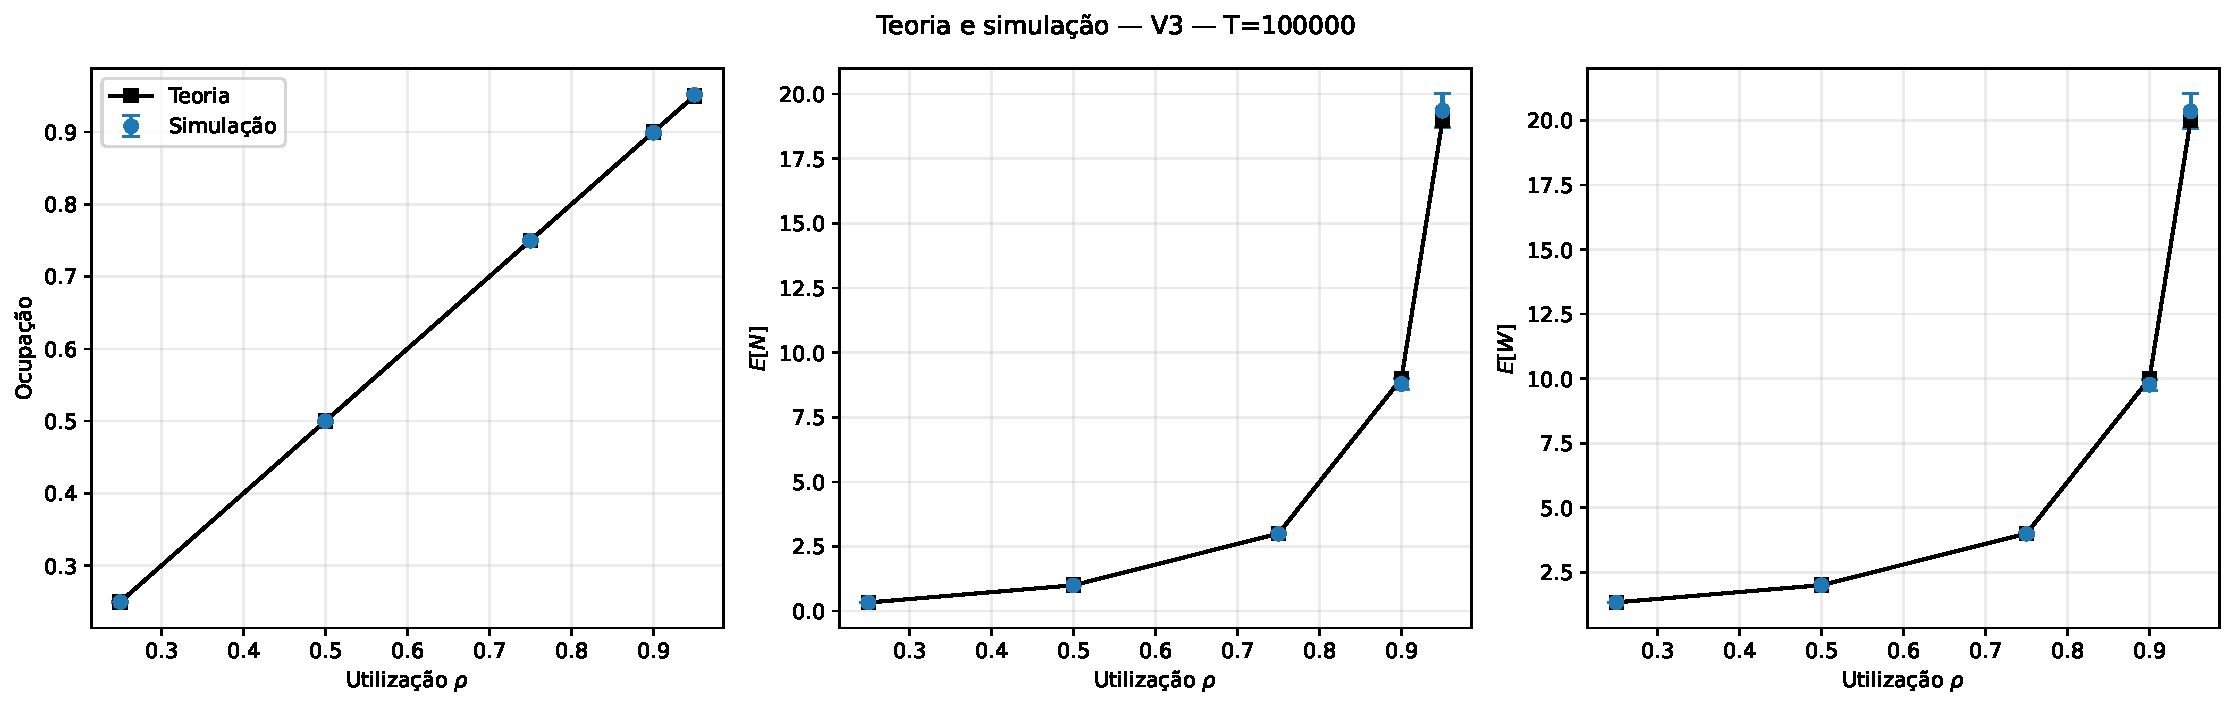
\includegraphics[width=0.95\textwidth]{imagem/teoria_simulacao_v3.pdf}
  \caption{Valores teóricos e simulados pela V3 para $T=10^5$.}
  \label{fig:teoria-simulacao}

  \vspace{2pt}
  {\footnotesize Fonte: elaboração própria.}
\end{figure}

A Tabela~\ref{tab:resultados-estaveis} apresenta os valores numéricos correspondentes. Em C1--C3, todos os erros relativos ficaram abaixo de 0,4\%. Em C4 e C5, as estimativas continuaram próximas da teoria, mas os erros de $\EN$ e $\EW$ aumentaram, atingindo cerca de 2,35\%. Esse comportamento é coerente com o crescimento da variabilidade e do tempo de convergência quando $\rho$ se aproxima de 1.

\begin{table}[H]
  \centering
  \caption{Resultados da V3 nos cenários estáveis para $T=10^5$.}
  \label{tab:resultados-estaveis}
  \resizebox{\textwidth}{!}{%
  \begin{tabular}{clrrrr}
    \toprule
    Cenário & Medida & Teórico & Média simulada & IC de 95\% & Erro relativo (\%) \\
    \midrule
    C1 & Ocupação & 0,2500 & 0,2497 & [0,2490; 0,2504] & 0,117 \\
    C1 & $\EN$    & 0,3333 & 0,3325 & [0,3310; 0,3341] & 0,243 \\
    C1 & $\EW$    & 1,3333 & 1,3301 & [1,3255; 1,3348] & 0,240 \\
    \midrule
    C2 & Ocupação & 0,5000 & 0,4999 & [0,4987; 0,5012] & 0,013 \\
    C2 & $\EN$    & 1,0000 & 0,9981 & [0,9919; 1,0044] & 0,187 \\
    C2 & $\EW$    & 2,0000 & 1,9967 & [1,9861; 2,0074] & 0,163 \\
    \midrule
    C3 & Ocupação & 0,7500 & 0,7495 & [0,7480; 0,7510] & 0,065 \\
    C3 & $\EN$    & 3,0000 & 2,9885 & [2,9545; 3,0225] & 0,382 \\
    C3 & $\EW$    & 4,0000 & 3,9865 & [3,9427; 4,0302] & 0,338 \\
    \midrule
    C4 & Ocupação & 0,9000 & 0,8990 & [0,8972; 0,9007] & 0,116 \\
    C4 & $\EN$    & 9,0000 & 8,7895 & [8,5884; 8,9907] & 2,338 \\
    C4 & $\EW$    & 10,0000 & 9,7651 & [9,5516; 9,9786] & 2,349 \\
    \midrule
    C5 & Ocupação & 0,9500 & 0,9513 & [0,9499; 0,9528] & 0,142 \\
    C5 & $\EN$    & 19,0000 & 19,3593 & [18,7033; 20,0154] & 1,891 \\
    C5 & $\EW$    & 20,0000 & 20,3568 & [19,6770; 21,0366] & 1,784 \\
    \bottomrule
  \end{tabular}}\par

  \vspace{2pt}
  {\footnotesize Fonte: elaboração própria.}
\end{table}

Os intervalos contêm os valores teóricos em C1, C2, C3 e C5 para as três medidas. Em C4, os limites superiores de $\EN$ e $\EW$ ficaram ligeiramente abaixo da teoria. Os dados disponíveis não permitem atribuir esse desvio a uma única causa. Flutuação amostral, inicialização vazia e truncamento da janela podem contribuir, mas não foi realizado um experimento que separe esses efeitos.

Na avaliação de 15 ICs individuais, mesmo que a cobertura nominal esteja correta, espera-se em média $15\times0{,}05=0{,}75$ intervalos que não contenham o valor de referência. Essa contagem esperada não exige independência entre as medidas e não determina a probabilidade conjunta das falhas. Como $\EN$ e $\EW$ de C4 compartilham acumuladores, as duas ausências de cobertura são relacionadas. O desvio é compatível com flutuação amostral, mas essa interpretação não exclui possíveis vieses e não permite atribuir uma causa definitiva.

\begin{table}[H]
  \centering
  \caption{Precisão relativa das médias da V3 para $T=10^5$.}
  \label{tab:precisao}
  \small
  \setlength{\tabcolsep}{4pt}
  \begin{tabular}{crrrc}
    \toprule
    Cenário & $h_r$ ocupação (\%) & $h_r$ de $\EN$ (\%) &
    $h_r$ de $\EW$ (\%) & \shortstack{Teoria nos\\três ICs?} \\
    \midrule
C1 & 0,29 & 0,46 & 0,35 & Sim \\
C2 & 0,25 & 0,63 & 0,53 & Sim \\
C3 & 0,20 & 1,14 & 1,10 & Sim \\
C4 & 0,20 & 2,29 & 2,19 & Não \\
C5 & 0,16 & 3,39 & 3,34 & Sim \\
    \bottomrule
  \end{tabular}\par
  \vspace{2pt}
  {\footnotesize Fonte: elaboração própria; semiamplitudes relativas dos ICs de 95\%.}
\end{table}

A Tabela~\ref{tab:precisao} distingue precisão de concordância com a teoria. Para C1 e C2, as semiamplitudes das três médias ficaram abaixo de 1\%. Em C3, as de $\EN$ e $\EW$ foram próximas de 1,1\%; em C4, cerca de 2,2\%; e em C5, cerca de 3,3\%. Embora o valor teórico esteja no IC de C5, sua média é menos precisa que a de C4. Portanto, cobertura do valor teórico e largura do intervalo respondem a perguntas diferentes. As tabelas completas das configurações podem ser consultadas no material complementar.

\subsection{Influência do horizonte de simulação}

A Figura~\ref{fig:convergencia} apresenta a evolução das médias da V3 nos cinco cenários estáveis. Os cenários crítico e sobrecarregado foram excluídos desse gráfico porque não possuem alvo estacionário e ampliariam a escala de $\EN$ e $\EW$, dificultando a leitura dos demais.

\begin{figure}[H]
  \centering
  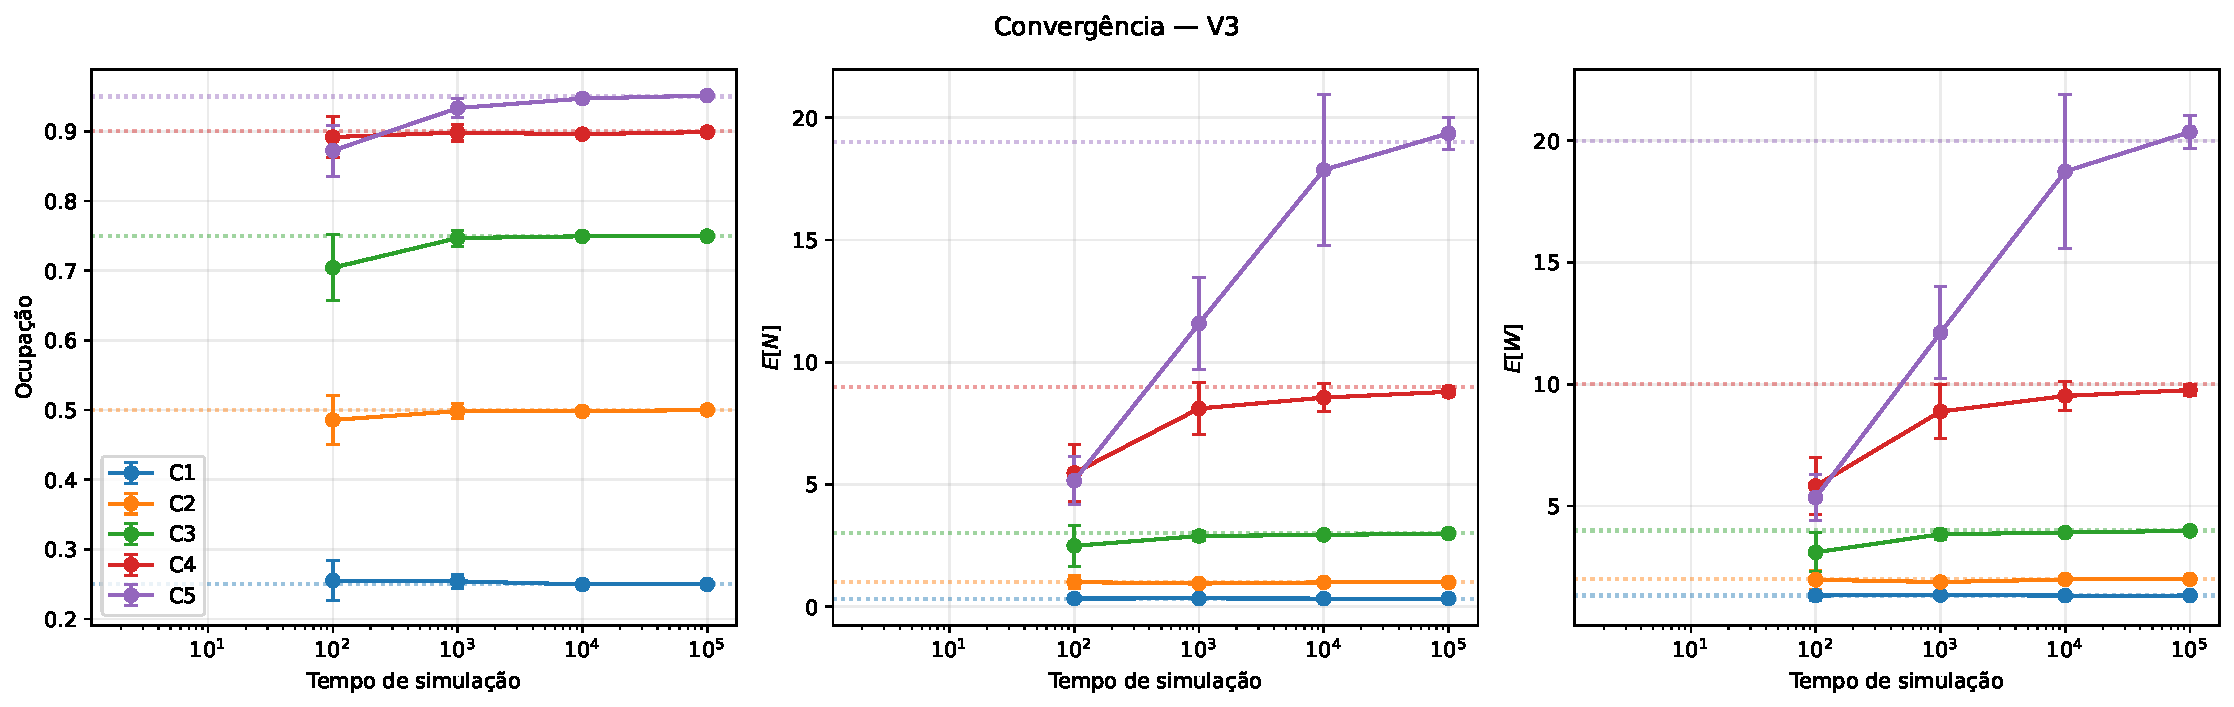
\includegraphics[width=0.97\textwidth]{imagem/convergencia_v3.pdf}
  \caption{Convergência das medidas da V3 em função do horizonte, com intervalos de confiança de 95\%.}
  \label{fig:convergencia}

  \vspace{2pt}
  {\footnotesize Fonte: elaboração própria.}
\end{figure}

No conjunto dos resultados, horizontes maiores produzem intervalos mais estreitos e melhor aproximação à teoria, especialmente quando comparados com as execuções mais curtas. Essa tendência não exige redução monotônica do erro em cada passagem de horizonte: sementes diferentes geram novas realizações, que podem ficar acima ou abaixo do alvo teórico. Uma execução longa contém mais eventos e reduz o peso proporcional da inicialização vazia, mas os dados não permitem quantificar separadamente esse viés. Em C4 e C5, os períodos de congestionamento são mais persistentes e as estimativas de $\EN$ e $\EW$ continuam mais variáveis. A convergência deve ser avaliada pelas médias e pela largura dos ICs, e não apenas pela forma das linhas que conectam os pontos.

\subsection{Variabilidade entre repetições}

A Figura~\ref{fig:boxplots} mostra as distribuições de $\EN$ e $\EW$ nas 30 repetições da V3 para $T=10^5$. Os dois painéis foram mantidos porque o número de solicitações e o tempo de permanência são medidas diferentes, embora relacionadas pela Lei de Little.

\begin{figure}[H]
  \centering
  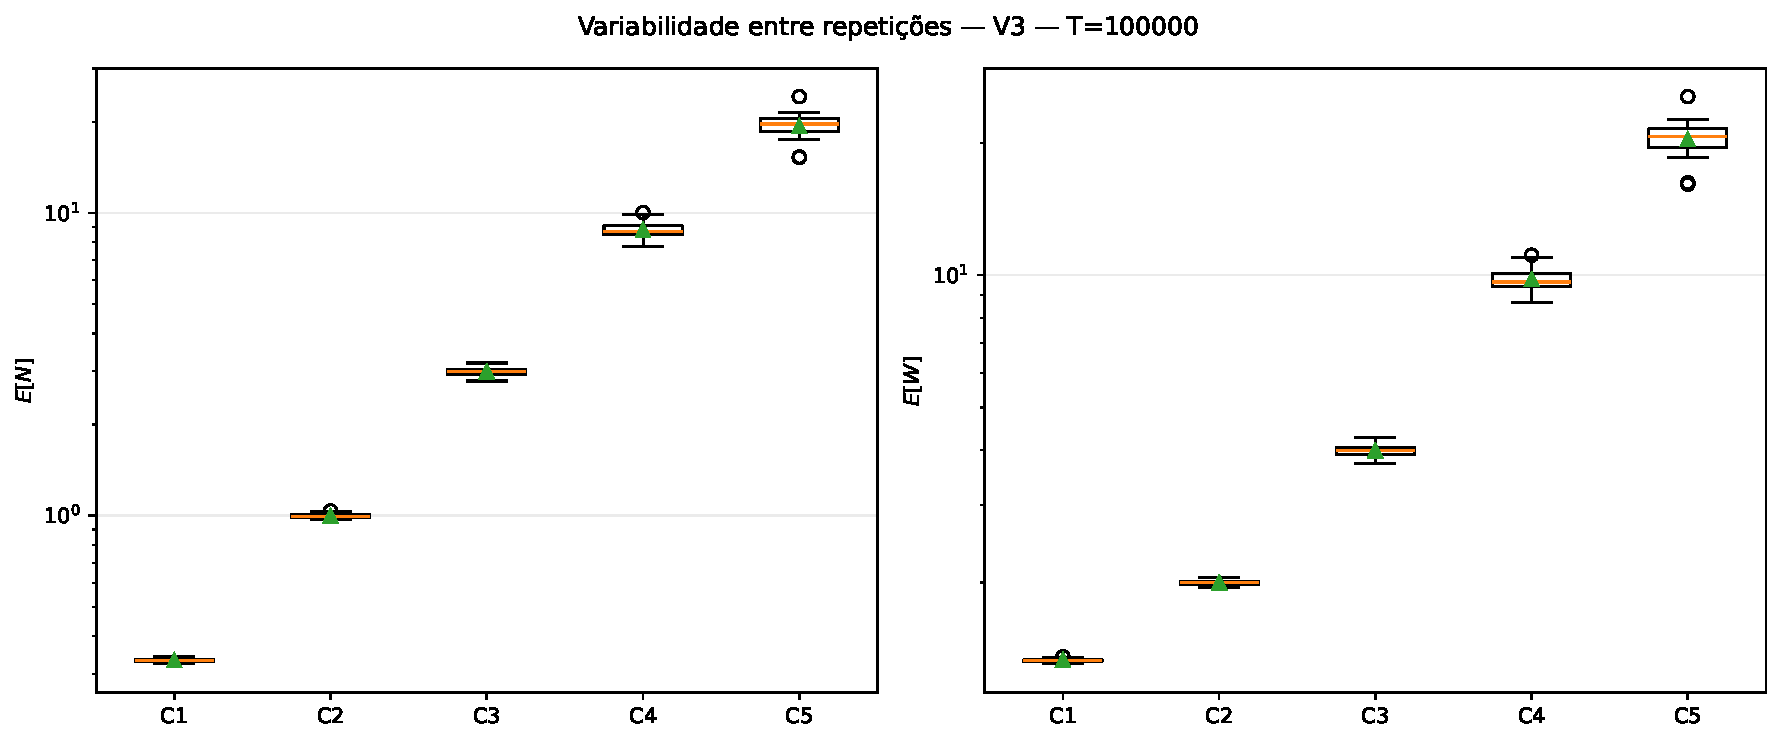
\includegraphics[width=0.96\textwidth]{imagem/boxplots_en_ew_v3.pdf}
  \caption{Distribuição de $\EN$ e $\EW$ entre as repetições da V3 para $T=10^5$.}
  \label{fig:boxplots}

  \vspace{2pt}
  {\footnotesize Fonte: elaboração própria.}
\end{figure}

Os boxplots mostram maior dispersão das estimativas conforme aumenta a carga. Em C1 e C2, os resultados ficam concentrados; em C4 e, principalmente, C5, a amplitude aumenta. Cada ponto utilizado no boxplot é uma média de uma execução, e não um tempo individual de cliente ou uma observação instantânea de $N(t)$. O gráfico descreve, portanto, a variabilidade entre repetições. Esse resultado justifica a apresentação de intervalos de confiança, pois a média isolada ocultaria a incerteza crescente perto de $\rho=1$.

\subsection{Taxa de chegada, vazão e saturação}

A Figura~\ref{fig:fluxo} compara a taxa de chegada observada com a vazão de saídas no maior horizonte. Essa verificação usa contagens de eventos e fornece uma análise complementar às áreas utilizadas em $\EN$ e $\EW$.

\begin{figure}[H]
  \centering
  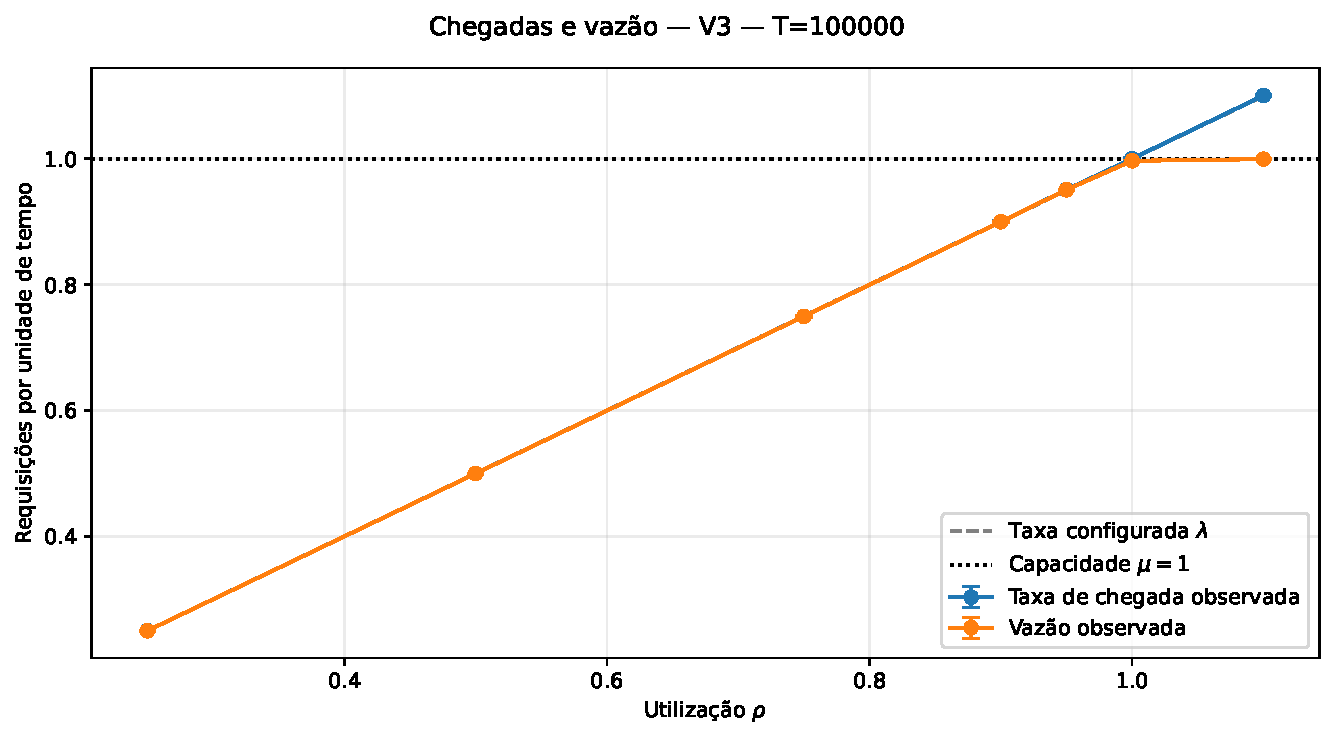
\includegraphics[width=0.88\textwidth]{imagem/fluxo_v3.pdf}
  \caption{Taxa de chegada observada e vazão da V3 para $T=10^5$.}
  \label{fig:fluxo}

  \vspace{2pt}
  {\footnotesize Fonte: elaboração própria.}
\end{figure}

Nos cenários estáveis, taxa de chegada e vazão praticamente coincidem, indicando que o sistema consegue processar a demanda no longo prazo. Em C7, a taxa observada foi aproximadamente 1,1005, enquanto a vazão ficou em 0,9994 solicitação por segundo, próxima da capacidade $\mu=1$. A diferença de cerca de 0,101 solicitação por segundo acumula-se no sistema. Em C6, pequenas flutuações entre chegadas e saídas também produzem acúmulo, pois não existe folga média de capacidade.

Para cada execução iniciada vazia, a conservação da população estabelece
\begin{equation}
  A(T_{\mathrm{obs}})-D(T_{\mathrm{obs}})=N(T_{\mathrm{obs}}),
  \qquad
  (\widehat{\lambda}-\widehat{v})T_{\mathrm{obs}}
  =N(T_{\mathrm{obs}}),
  \label{eq:conservacao-fluxo}
\end{equation}
em que $\widehat{v}$ é a vazão observada. A segunda igualdade foi conferida nos 1.680 registros do CSV: o maior resíduo absoluto ficou abaixo de $10^{-7}$ solicitação, compatível com o arredondamento das taxas impressas. Trata-se de outra verificação de consistência interna, baseada em fluxo e população, que complementa a análise das áreas sem substituir a comparação com a teoria. Em C7, a diferença de taxas, multiplicada pelo tempo observado, explica a população final próxima de dez mil solicitações.

\subsection{Tratamento do horizonte na V3}

A Figura~\ref{fig:excesso-horizonte} mostra a diferença média entre o tempo final processado e o horizonte solicitado na V3. O excesso foi positivo nas configurações avaliadas, confirmando empiricamente o problema de encerramento identificado na leitura do código.

\begin{figure}[H]
  \centering
  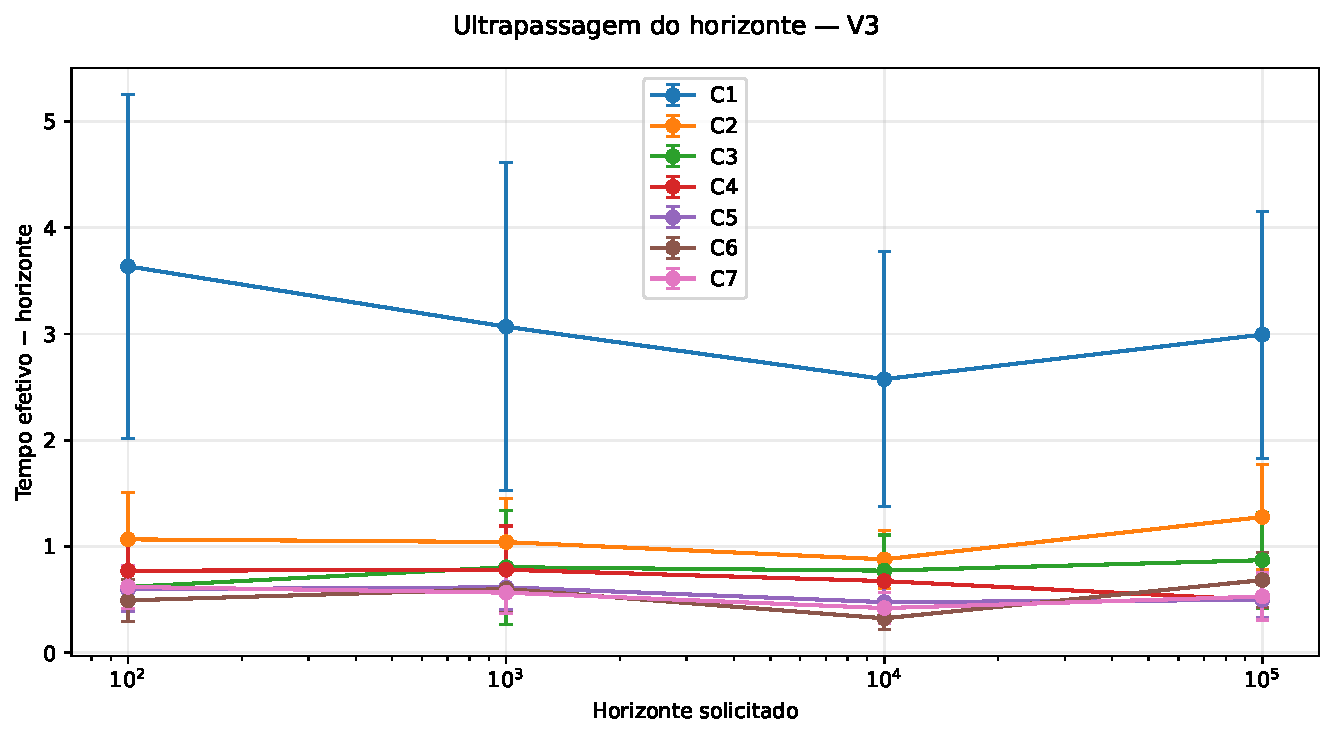
\includegraphics[width=0.90\textwidth]{imagem/excesso_horizonte_v3.pdf}
  \caption{Excesso médio do tempo final sobre o horizonte solicitado na V3.}
  \label{fig:excesso-horizonte}

  \vspace{2pt}
  {\footnotesize Fonte: elaboração própria.}
\end{figure}

O excesso absoluto depende do intervalo até o primeiro evento posterior ao limite e, por isso, não precisa desaparecer quando $T$ aumenta. Seu peso relativo, entretanto, diminui. Por exemplo, em C1 a média do excesso foi aproximadamente 3,64 segundos para $T=100$ e 2,99 segundos para $T=10^5$; proporcionalmente, o primeiro caso é muito mais afetado. A V4 interrompe o relógio exatamente em $T$ e fecha as áreas nesse instante, eliminando esse desvio.

\subsection{Cenários crítico e sobrecarregado}

A Figura~\ref{fig:populacao-final} apresenta a população final em função de $\rho$, mantendo o horizonte como séries distintas. O eixo principal é a carga porque o objetivo é evidenciar a transição entre os regimes estável, crítico e sobrecarregado.

\begin{figure}[H]
  \centering
  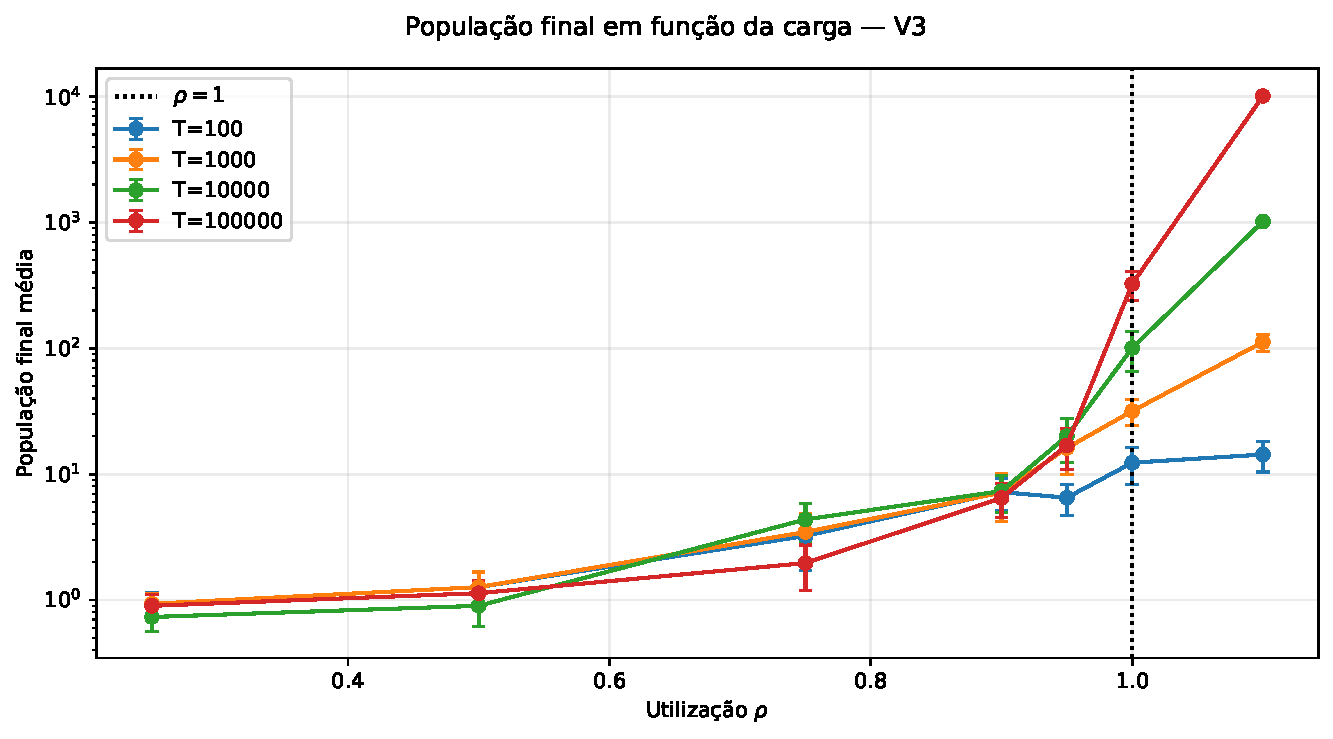
\includegraphics[width=0.90\textwidth]{imagem/populacao_final_rho_v3.pdf}
  \caption{População final da V3 em função de $\rho$ para diferentes horizontes.}
  \label{fig:populacao-final}

  \vspace{2pt}
  {\footnotesize Fonte: elaboração própria.}
\end{figure}

Em C1--C5, a população final permanece relativamente limitada no conjunto de horizontes, embora aumente perto da saturação. Ela é uma observação do encerramento e pode ser elevada mesmo em um cenário estável; não deve ser confundida com $\EN$, que é uma média temporal.

Em C6, as médias da população final foram 12,33, 31,73, 100,77 e 324,87 para $T=10^2$, $10^3$, $10^4$ e $10^5$, respectivamente. Nos três maiores horizontes, a razão $\bar{N}_{\mathrm{final}}/\sqrt{T}$ ficou entre 1,00 e 1,03. Esse padrão é compatível com crescimento na escala de $\sqrt{T}$ e difere do crescimento aproximadamente linear do cenário sobrecarregado. A comparação é descritiva e utiliza quatro horizontes; não constitui um ajuste estatístico nem uma determinação exata da lei de crescimento.

Em C7, a população final média passou de 14,33 em $T=100$ para 10.107,07 em $T=10^5$. O último valor é próximo de $(\lambda-\mu)T=10.000$, coerente com o excesso médio de demanda de 0,1 solicitação por segundo. Esses resultados descrevem janelas finitas e não são estimativas de médias estacionárias.

\subsection{Lei de Little}

A Tabela~\ref{tab:little} resume o valor absoluto do resíduo $\varepsilon_L=\widehat{\EN}-\widehat{\lambda}\widehat{\EW}$ em todas as 840 execuções de cada versão. As médias são da ordem de $10^{-11}$ e os máximos, de $10^{-9}$, refletindo erros numéricos de ponto flutuante e o arredondamento das saídas.

\begin{table}[H]
  \centering
  \caption{Resíduo absoluto da Lei de Little nas execuções.}
  \label{tab:little}
  \begin{tabular}{lcc}
    \toprule
    Versão & Média de $|\varepsilon_L|$ & Máximo de $|\varepsilon_L|$ \\
    \midrule
    V3 & $6{,}42\times10^{-11}$ & $1{,}18\times10^{-9}$ \\
    V4 & $8{,}79\times10^{-11}$ & $2{,}05\times10^{-9}$ \\
    \bottomrule
  \end{tabular}\par

  \vspace{2pt}
  {\footnotesize Fonte: elaboração própria.}
\end{table}

O resultado confirma que os acumuladores internos preservam a identidade utilizada no cálculo. Contudo, como $\EN$ e $\EW$ são derivados das mesmas áreas, um resíduo quase nulo não demonstra sozinho que ambas as médias estão corretas. A concordância com as fórmulas teóricas nos cenários estáveis e a compatibilidade entre taxa de chegada, vazão e população final fornecem evidências adicionais e menos circulares.

\subsection{Efeito das correções da V4}

A Figura~\ref{fig:comparacao-versoes} apresenta a média das diferenças assinadas V3$-$V4 e os ICs pareados de 95\%, calculados por cenário e horizonte com números aleatórios comuns. Um IC que contém zero indica que a diferença média não foi distinguida de zero pelo procedimento adotado; um IC que não contém zero indica uma diferença detectável, cuja importância prática ainda depende de sua magnitude.

A Tabela~\ref{tab:diferencas-versoes} resume outra quantidade: a média de $|d_r|$ nos 150 pares de cada horizonte, reunindo os cinco cenários estáveis com 30 repetições cada. Ela expressa o tamanho médio das diferenças sem cancelamento de sinais e não é um IC pareado.

\begin{figure}[H]
  \centering
  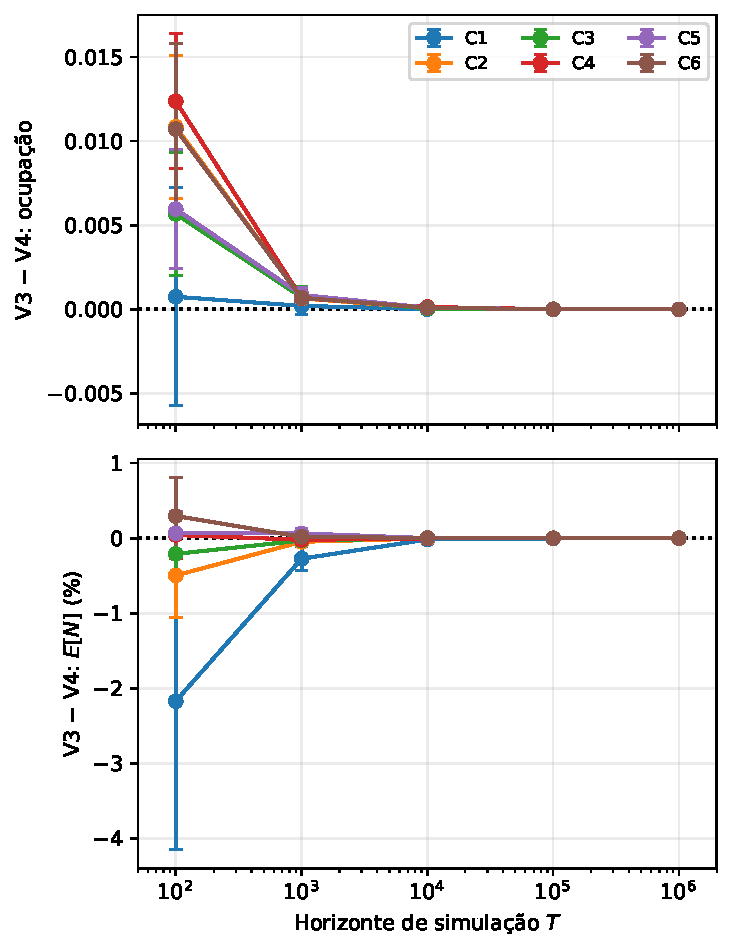
\includegraphics[width=0.97\textwidth]{imagem/comparacao_v3_v4.pdf}
  \caption{Comparação pareada entre V3 e V4 nos diferentes horizontes.}
  \label{fig:comparacao-versoes}

  \vspace{2pt}
  {\footnotesize Fonte: elaboração própria.}
\end{figure}

\begin{table}[H]
  \centering
  \caption{Diferença absoluta média entre V3 e V4 nos cenários C1--C5.}
  \label{tab:diferencas-versoes}
  \begin{tabular}{rccc}
    \toprule
    Horizonte & Ocupação & $\EN$ & $\EW$ \\
    \midrule
    $10^2$ & 0,010652 & 0,017082 & 0,040145 \\
    $10^3$ & 0,001029 & 0,003604 & 0,007105 \\
    $10^4$ & 0,000099 & 0,000287 & 0,000611 \\
    $10^5$ & 0,000009 & 0,000027 & 0,000057 \\
    \bottomrule
  \end{tabular}\par

  \vspace{2pt}
  {\footnotesize Fonte: elaboração própria.}
\end{table}

As diferenças são maiores em execuções curtas, nas quais o tratamento do evento posterior ao limite possui maior peso proporcional. Em $T=10^5$, as diferenças absolutas médias ficam na ordem de $10^{-5}$ para ocupação e população e de $10^{-5}$ a $10^{-4}$ para permanência. Algumas diferenças assinadas continuam estatisticamente detectáveis, mas sua magnitude é pequena diante das próprias medidas. Portanto, uma diferença detectável não implica necessariamente uma alteração importante no desempenho estimado.

As duas versões usam o mesmo gerador e a mesma lógica de sorteios para os eventos compartilhados anteriores ao horizonte. A V3 ainda processa o primeiro evento posterior e pode realizar sorteios adicionais nessa fronteira; a V4 encerra em $T$. O pareamento reduz a influência de trajetórias diferentes e permite relacionar as discrepâncias às correções de encerramento e ocupação. Os resultados sustentam a coerência da dinâmica central da V3 nas configurações avaliadas e mostram o benefício da V4 para definir uma janela de observação consistente.

% ================================================================
% 6 CONSIDERAÇÕES FINAIS
% ================================================================

\section{Considerações finais}

Este trabalho analisou o funcionamento de um simulador M/M/1, relacionou sua implementação aos fundamentos de teoria de filas e avaliou seu comportamento em diferentes cargas e horizontes. O experimento combinou sete cenários, quatro durações e 30 repetições, permitindo discutir não apenas médias, mas também incerteza, convergência, conservação de fluxo, saturação e limitações do código.

Nos cenários estáveis, os horizontes maiores ofereceram, no conjunto, melhor aproximação à teoria e intervalos mais estreitos. Para $T=10^5$, C1--C3 apresentaram erros inferiores a 0,4\%, enquanto C4 e C5 tiveram erros de até aproximadamente 2,35\% para população e permanência. A precisão relativa também variou: as semiamplitudes dessas medidas ficaram abaixo de 1\% em C1 e C2 e ultrapassaram 3\% em C5. A ausência de cobertura da teoria em duas medidas relacionadas de C4 foi interpretada com cautela, sem atribuição conclusiva ao transiente inicial.

A análise de fluxo mostrou que chegadas e saídas se equilibram quando $\rho<1$, enquanto a vazão se limita à capacidade do servidor no cenário sobrecarregado. A população final crescente em C6 e C7 demonstrou por que não se devem aplicar fórmulas estacionárias quando $\rho\geq1$. O resíduo de Little permaneceu numericamente próximo de zero, mas foi interpretado como uma identidade interna dos acumuladores e não como prova independente da correção do simulador.

A comparação pareada confirmou diferenças maiores nos horizontes curtos e pequenas em magnitude nas execuções longas. A V4 encerrou exatamente no horizonte solicitado e ajustou a contabilização da ocupação na janela. Esses resultados mostram que a correção de fronteira melhora a definição da observação, mesmo quando sua influência prática nas médias de longo prazo é pequena.

O início vazio, a ausência de aquecimento, o cálculo truncado de $W$ e a falta de avaliação estatística do gerador limitam as conclusões. O registro incompleto do ambiente também restringe a reprodução numérica entre máquinas. A coleta de tempos individuais poderia ampliar a análise e permitir uma verificação independente da Lei de Little. Nas condições estudadas, o simulador reproduz os principais comportamentos de uma fila M/M/1. Sua validação, porém, exige observar conjuntamente a concordância com a teoria, a precisão das estimativas e a forma como o código mede cada grandeza.

% ================================================================
% REFERÊNCIAS
% ================================================================

\section*{Referências}
\addcontentsline{toc}{section}{Referências}

\begin{spacing}{1.0}
\raggedright

\noindent
GONZAGA, Flávio Barbieri. \textbf{Análise de desempenho: aulas 1 a 7}.
Alfenas: Universidade Federal de Alfenas, 2026. Material didático em slides.

\vspace{0.5em}

\noindent
KENDALL, David G. Stochastic processes occurring in the theory of queues and
their analysis by the method of the imbedded Markov chain. \textbf{The Annals
of Mathematical Statistics}, v. 24, n. 3, p. 338--354, 1953. DOI:
\url{https://doi.org/10.1214/aoms/1177728975}.

\vspace{0.5em}

\noindent
LITTLE, John D. C. A proof for the queuing formula: $L=\lambda W$.
\textbf{Operations Research}, v. 9, n. 3, p. 383--387, 1961. DOI:
\url{https://doi.org/10.1287/opre.9.3.383}.

\vspace{0.5em}

\noindent
ROSS, Sheldon M. \textbf{Simulation}. 4. ed. San Diego: Academic Press, 2006.

\vspace{0.5em}

\noindent
TRIVEDI, Kishor S. \textbf{Probability and statistics with reliability,
queuing, and computer science applications}. 2. ed. New York: John Wiley
\& Sons, 2001.

\end{spacing}


\end{document}
